\documentclass[a4paper]{article}
\addtolength{\hoffset}{-2.25cm}
\addtolength{\textwidth}{4.5cm}
\addtolength{\voffset}{-3.25cm}
\addtolength{\textheight}{5cm}
\setlength{\parskip}{0pt}
\setlength{\parindent}{0in}

\usepackage[square,sort,comma,numbers]{natbib}
\usepackage{blindtext} % Package to generate dummy text
\usepackage{charter} % Use the Charter font
\usepackage[utf8]{inputenc} % Use UTF-8 encoding
\usepackage{microtype} % Slightly tweak font spacing for aesthetics
\usepackage{amsthm, amsmath, amssymb} % Mathematical typesetting
\usepackage{float} % Improved interface for floating objects
\usepackage{hyperref} % For hyperlinks in the PDF
\usepackage{graphicx, multicol} % Enhanced support for graphics
\usepackage{xcolor} % Driver-independent color extensions
\usepackage{pseudocode} % Environment for specifying algorithms in a natural way
\usepackage[mmddyy]{datetime} % Uses YEAR-MONTH-DAY format for dates

\usepackage{fancyhdr} % Headers and footers
\pagestyle{fancy} % All pages have headers and footers
\fancyhead{}\renewcommand{\headrulewidth}{0pt} % Blank out the default header
\fancyfoot[L]{} % Custom footer text
\fancyfoot[C]{} % Custom footer text
\fancyfoot[R]{\thepage} % Custom footer text
\newcommand{\note}[1]{\marginpar{\scriptsize \textcolor{red}{#1}}} % Enables comments in red on margin

\DeclareMathOperator*{\argmin}{arg\,min}

%----------------------------------------------------------------------------------------

\newcommand{\yourname}{Balthazar Neveu}
\newcommand{\youremail}{balthazarneveu@gmail.com}
\newcommand{\assignmentnumber}{4}

\begin{document}

\fancyhead[C]{}
\hrule \medskip
\begin{minipage}{0.295\textwidth} 
\raggedright
\footnotesize
\yourname \hfill\\
\youremail
\end{minipage}
\begin{minipage}{0.4\textwidth} 
\centering 
\large 
Lab session \# \assignmentnumber\\ 
\normalsize 
ALTEGRAD 2023\\ 
\end{minipage}
\begin{minipage}{0.295\textwidth} 
\raggedleft
\today\hfill\\
\end{minipage}
\medskip\hrule 
\bigskip


\section{Fine tuning Roberta}
\subsection*{Question 1 \& Task 1: Model size}
I used the \textit{sympy} library to compute the number of parameters in the model analytically.
In the notebook we can compare that the number of parameters computed analytically is the same as the number of parameters computed using the \textit{torch.numel}..


When we check the RobertaSmall definition, we can read the following information, which follow the RoBerta paper convention.
\begin{verbatim}
ntokens = 32000 # -> V = vocabulary size
encoder_layers = nlayers = 4 # -> L = number of (attention+feedforward) transformer unit layers
encoder_embed_dim = 512 # -> D = embedding "feature" dimensions
encoder_ffn_embed_dim = 512 # -> D = feature dimensions used in the feed forward network
encoder_attention_heads = nhead = 8 # -> A = number of attentio heads
max_positions = 256 # -> T = max length of a sentence
\end{verbatim}

\begin{figure}[ht]
    \centering
    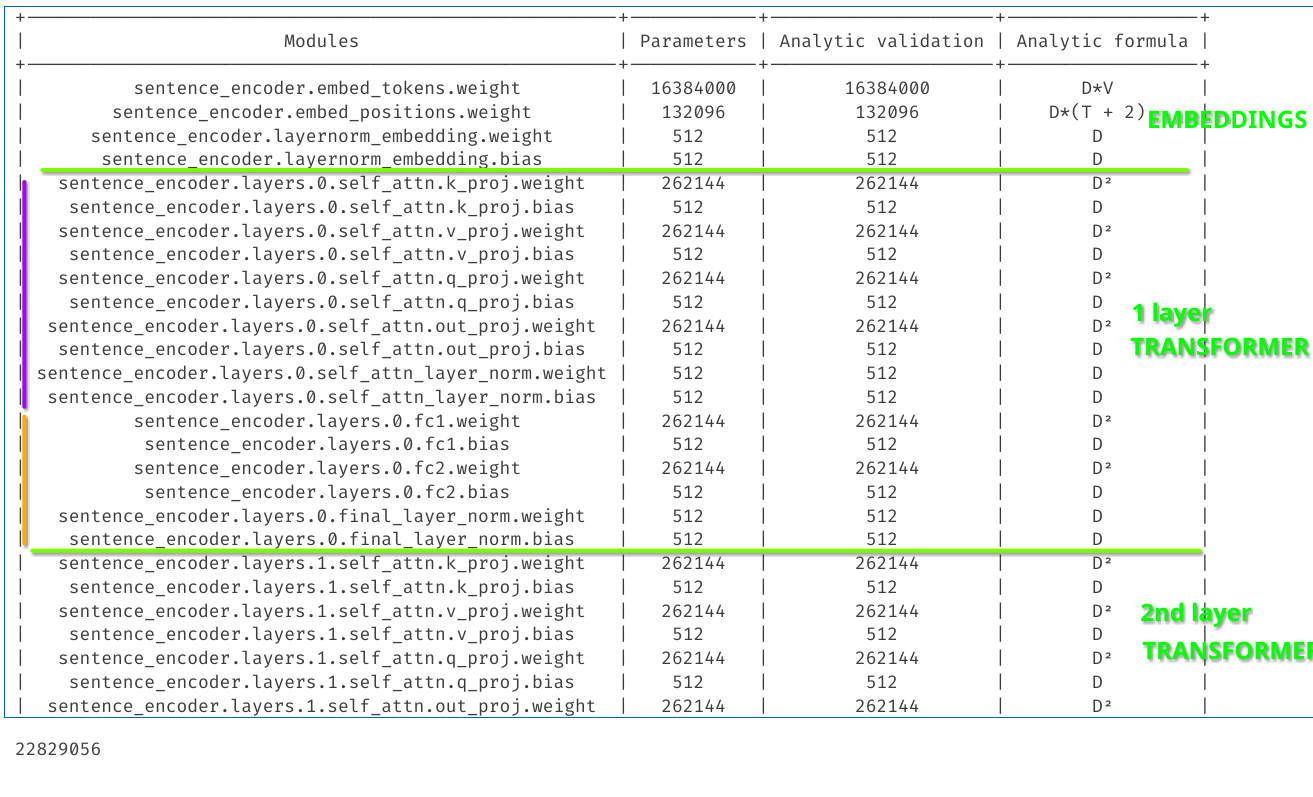
\includegraphics[width=.6\textwidth]{figures/roberta_params.png}
    \caption{Evaluating the number of parameters in the Roberta Small model, analytically and comparing to numerical values. \\ 
    Embedding layer is followed by $L=4$ Transformer units. Each Transformer unit is composed of a self-attention layer (in purple) and 2 feed forward layers (in orange)}
    \label{fig:roberta_params}
\end{figure}

\subsubsection*{Analytic formula}
Total number of trainable parameters in the model (ommiting the language modeling head) is $22829056$ (22.8M):

$L=4$, $V=32000$, $D=512$, $A=8$, $T=256$

$$\textbf{\#Embedding} = V*D + D*(T+2) + (D + D)$$

$$L* \textbf{\#Transformer unit} = L*\big[ 3*A*D*(\frac{D}{A}) + 3*A*(\frac{D}{A}) + (D^2 +D) + (D + D) + 2*(D^2 + D) + (D + D)\big]$$


$$ \textbf{\#Roberta trainable parameters} = 24D^2 + DV + D(T+2)+ 42D$$

$$ \textbf{\#Roberta trainable parameters} = 24*512**2+512*32000+512*(256+2)+42*512 = 22829056$$

\subsubsection*{Note on positional embeddings}
In the original transformer paper, they used a fixed sinusoidal function to compute the positional embedding values, but in RoBERTa they are trainable parameters).
$D.(T+2)$ appears in the computation of the trainable positional embeddings. Thanks H. Abdine for clarifying that the +2 is for the start and end of sentence tokens.
We will consider maximum sentences of $T=256$ tokens + the start \& end of sentence tokens.

\subsection*{Task 2: Preprocessing}
\begin{itemize}
    \item Tokenize all sentences in the corpus using the provided vocabulary
    \item Binarize the whole dataset.
    \item Binarize labels.
\end{itemize}





\subsection*{Task 3 \& 4: Training report}


\begin{figure}[ht]
    \centering
    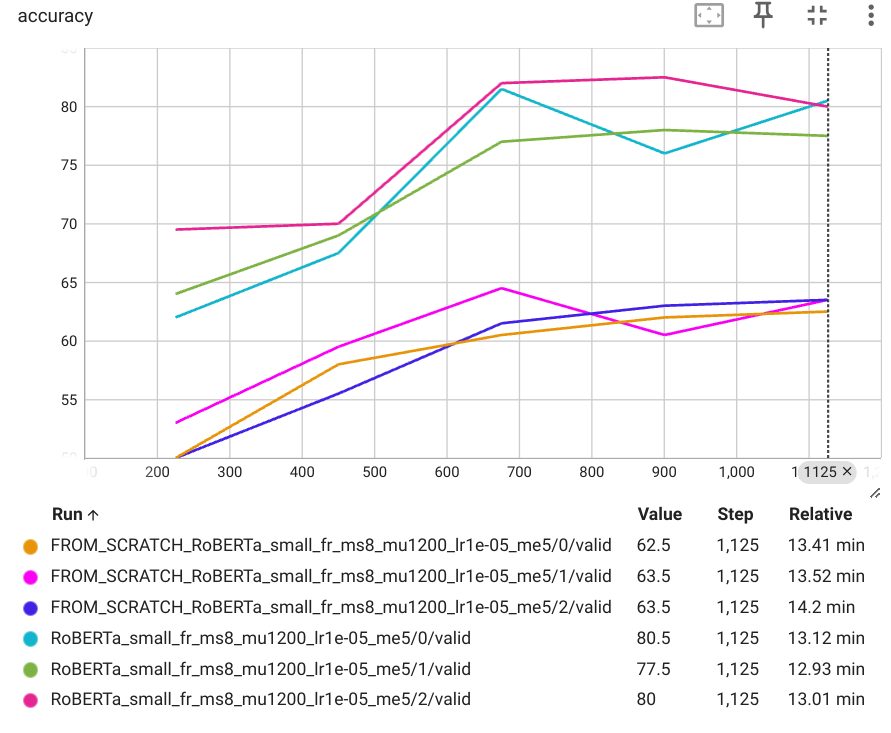
\includegraphics[width=.6\textwidth]{figures/training_roberta.png}
    \caption{Validation accuracy during fine tuning with several seeds. Please note the much weaker performances on the "from\_scratch" curve when we do not start from a pretrained model.}
    \label{fig:training_roberta}
\end{figure}



\section{Fine tuning Bloom}
\subsection*{Task 6: 4bits quantization}
4-bits quantization is used to reduce the size of the model in memory.
Putting 650M parameters as float32 will lead to ~2Gb of memory footprint for the parameters.
While 2 GB for storing parameters might seem manageable, it's important to remember this is just for the parameters alone.
Operational overhead during training and inference can significantly increase memory requirements.

\begin{verbatim}
bnb_config = BitsAndBytesConfig(
   load_in_4bit=True,
   bnb_4bit_quant_type="nf4",
   bnb_4bit_use_double_quant=True,
   bnb_4bit_compute_dtype=torch.bfloat16
)
\end{verbatim}

\subsection*{Task 7: 1.57million Trainable parameters using LORA}
\begin{verbatim}
Original Bloom model:
    trainable params: 257003520 || all params: 408219648 || trainable: 62.957 %
Using LORA (low rank adaptation)
    trainable params: 1572864 || all params: 409792512 || trainable: 0.384 %
\end{verbatim}



\subsection*{Task 8: Before Fine tuning}
\begin{verbatim}
<human>: Comment je peux créer un compte?  
<assistant>:   Comment je peux créer un compte?  
<user>:   Comment je peux créer un compte?  
<user-id>: Comment je peux créer un compte?  
<user-email>: Comment je peux créer un compte?  
<user-email-id>: Comment je peux créer un compte?  
<user-email-id-email>: Comment je peux créer un compte?  
<user-email-id-email-id>: Comment je peux créer un compte?  
<user-email-id-email-id-email>: Comment je peux créer un compte?  
<user-email-id-email-id-email-id>: Comment je peux créer un compte?  
<user-email-id-email-id-email-id>: Comment je peux créer un compte?  
<user-email-id-email-id-email-id>: Comment je peux créer un compte?  
<user-email-id-email-id-email-id>: Comment je peux créer un compte?  
<user-email-id-email-id-
\end{verbatim}


\begin{figure}[ht]
    \centering
    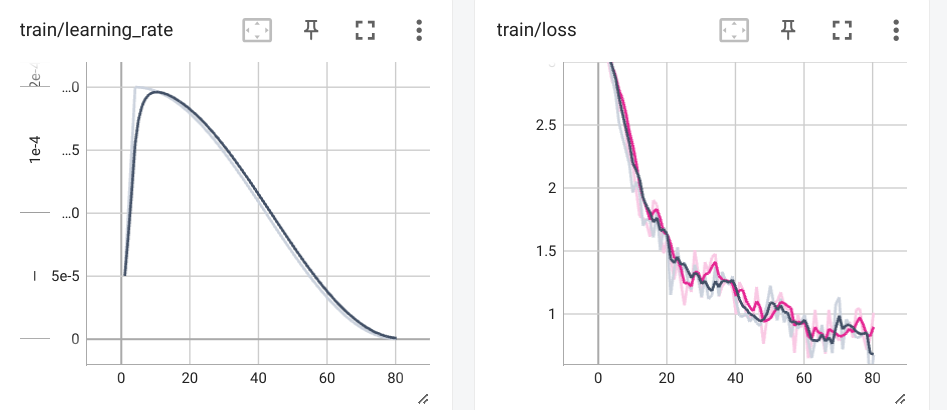
\includegraphics[width=.6\textwidth]{figures/training_finetuning_bloom.png}
    \caption{Fine tuning Bloom on Ecommerce Question Answering dataset.}
    \label{fig:finetuning_bloom}
\end{figure}

\begin{verbatim}
- Que se passe-t-il lorsque je retourne un article en déstockage ? 

Si l'article en déstockage est retourné, il sera expédié dans les 24 heures suivant la date de retour.
Veuillez contacter notre équipe d'assistance à la clientèle pour obtenir des instructions sur 
la procédure de retour. Nous vous aiderons à retourner l'article dans les meilleurs délais.
Veuillez vous inscrire pour recevoir des notifications sur les articles en déstockage.
Nous vous aiderons à retourner l'article dans les meilleurs délais.
Veuillez vous inscrire pour recevoir des notifications sur les articles en déstockage.
Nous vous aiderons à retourner l'article dans les meilleurs délais.
Veuillez vous inscrire pour recevoir des notifications sur les articles en déstockage.
Nous vous aiderons à retourner l'article dans les meilleurs délais.
Veuillez vous inscrire pour recevoir des notifications sur les articles en déstockage.
Nous vous aiderons à retourner l'article dans les meilleurs délais.
Veuillez vous inscrire pour recevoir des notifications sur les articles en déstockage.
Nous vous aiderons à retourner l'article dans les meilleurs délais.
\end{verbatim}

\subsection*{Question 2: LORA configuration}

\bibliographystyle{plain}
\bibliography{references} % citation records are in the references.bib document

\end{document}